\section{Using FADAtool}
The following sections explain the input and the output of \verb|FADAtool|. This command line tool has many options explained when executing \verb|FADAtool -h| or \verb|FADAtool --help|. 
\subsection{Input Program Format}
\verb|FADAtool| takes a C program as input by using the option \verb|-i program_name.c|. However, we do not handle all the C language. Our frontend parser has the following limitations:
\begin{itemize}
 \item User defined types are supported only with simple {\texttt typedef} declarations.
 \item C for-loops are considered as regular static for-loops with a simple stride counter, upper and lower bounds. More complicated shapes of C-for loops are not handled.
 \item Pre and Post-increment operators are not allowed within expressions.
 \item Out input C language support special \verb|#pragma fada| used to declare any static assertion helping the code analysis. This pragma is attached to the statement just after it. Other pragmas are not supported, and the current version of the tool may crash if other pragmas are used!
\end{itemize}
To better understand our C subset used as input format to \verb|FADAtool|, we invite the reader to study the program examples delivered with source codes package of FADA. 
\subsection{Output}
This section illustrates the outputs of \verb|FADAtool|, which are data flow dependences (quasts). In addition to the console output, \verb|FADAtool| can generate HTML pages if appropriate tools have been installed, see Section~\ref{fada_prerequis}). The HTML pages contain exactly the same information printed on the console, but in a better look.

\subsubsection{The Console Output}
First, we show some output result for standard static control programs. For non static control programs, data dependences are more complex, so the output is also complex. Let start by illustrating the output of \verb|FADAtool| executed on a static control program, then we explain how things change in case of non static control programs.

%\paragraph{Static Control Programs}
\paragraph{Static Control Programs}
\begin{figure}[!h]
\begin{footnotesize}
\begin{lstlisting}
void    MatrixMultiply(int A[N][L], int B[L][M], int T[N][M]){
int i;
int j;
int k;
for(i=0;i<N;i++)
   for(j=0;j<M;j++){
        T[i][j]=0;
        for(k=0;k<L;k++)
                T[i][j]+=A[i][k]*B[k][j];
        }
\end{lstlisting}
\end{footnotesize}
\caption{\texttt{MatMul.c}: Static Control Program Example}
\label{pgm:matmul}
\end{figure}




\begin{figure}[!h]
\begin{scriptsize}
\begin{verbatim}
 $ fadatool -i MatMul.c
/////////////////////////////////////////////////
Symbolic constants are  = ( N, M, L )
/////////////////////////////////////////////////
********************************************
ID		:0
Counters	:(  )
Domain		:true
Written variable:
Read variable:
********************************************
ID		:1
Counters	:( i )
Domain		:((i >= 0) and (i <= N-1))
Written variable:
Read variable:
********************************************
ID		:2
Counters	:( i, j )
Domain		:(((i >= 0) and (i <= N-1))) and ((j >= 0) and (j <= M-1))
Written variable:   T[ i ][ j ]
Read variable:
********************************************
ID		:3
Counters	:( i, j )
Domain		:(((i >= 0) and (i <= N-1))) and ((j >= 0) and (j <= M-1))
Written variable:
Read variable:
********************************************
ID		:4
Counters	:( i, j, k )
Domain		:((((i >= 0) and (i <= N-1))) and ((j >= 0) 
                                  and (j <= M-1))) and ((k >= 0) and (k <= L-1))
Written variable:   T[ i ][ j ]
Read variable:
   T[ i ][ j ]

         if ( k >= 1 )
            < 4 : i, j, k-1 > 
         else
            < 2 : i, j >

   A[ i ][ k ]
      _|_

   B[ k ][ j ]
      _|_

/////////////////////////////////////////////////
================ Parallel Loops Detector:
      Parallel loops are : ( i, j ) 
================================
\end{verbatim}
\end{scriptsize}
\caption{Console Output for Dataflow Analysis of \texttt{MatMul.c} (Figure~\ref{pgm:matmul})}
\label{output:matmul}
\end{figure}

\verb|FADAtool| starts by detecting the symbolic constants of the program (first line in Figure~\ref{output:matmul}). Then it computes the guarded references from the statements of the original program. In fact, \verb|FADAtool| does not need the AST of the program. The required information are:
\begin{itemize}
 \item Which variables are read and written,
 \item within which loops (defined by their counters),
 \item and, what is the condition for which these variables can be read and written.
\end{itemize}

For example, the second assignment (\verb|ID#4|) reads three references (\verb|T[i][j]|, \verb|A[i][k]|, and \verb|B[k][j]|), one is written (\verb|T[i][j]|). These references are enclosed by loops \verb|i, j, k|, and guarded by the domain condition: ($ 0 \leq i \leq N-1,  0 \leq j \leq M-1, 0 \leq k \leq L-1$).

For each read variable, \verb|FADAtool| computes its source and expresses it in a quast. So, the definition of \verb|T[i][j]| read by \verb|ID#4| during iteration \verb|(i, j, k)| is (also given in Figure~\ref{output:matmul}):


\begin{verbatim}
         if ( k >= 1 )
            < 4 : i, j, k-1 > 
         else
            < 2 : i, j >
\end{verbatim}

And the source of \verb|A[i][j]| (read by \verb|ID#4| during the iteration \verb|(i, j, k)|) is :
\begin{verbatim}
      _|_
\end{verbatim}
In the console output, $\perp$ or Bottom  means that the source is undefined (out of analysedyzed scope). \verb|<ID : ITERATION_VECTOR >|  means that the value was produced by the statement \verb|ID|, during the iteration \verb|ITERATION_VECTOR|.


The exact source are computed by \verb|FADAtool| for \verb|T[i][j]|. It is presented as a quast, and should be read as : if \verb|A[i][j]| is read during the first iteration of the \verb|k|-loop, so its value is produced by assignment \verb|ID#2|. Otherwise, it its value is produced by assignment \verb|ID#4| executed during the previous iteration of the \verb|k|-loop, but int the same \verb|i-j|-loop iteration.


The third part of the output plots the parallel loops. Out parallel loops detector is elementary, it considers loops which do not carry dependences. This part is under constant improvments.

%\paragraph{Non Static Control Programs}
\paragraph{Non Static Control Programs}
\begin{verbatim}
 $ fadatool -i max.c
\end{verbatim}

\begin{figure}[!h]
\begin{footnotesize}
 \begin{verbatim}
   int Max(int N, int *V){
      int max
      int i;
      max=V[0];
      for(i=1;i<N;i++)
         if(max < V[i])
            max=V[i];
      return(max);
      }
 \end{verbatim}
\begin{center}
\begin{scriptsize}
\end{scriptsize}
\end{center}

\end{footnotesize}
\caption{{\texttt max.c}: Computing the Maximum of a Vector}
\label{pgm:max_vect}
\end{figure}
The example in Figure~ \ref{pgm:max_vect} is a non static control program, because of the existence of a control (\verb|if|) with non affine condition.
If we look at the source of \verb|max| read by the last statement, we get thanks to \verb|FADAtool|:
\begin{verbatim}
   max
         if ( (i_3_0 >= 1) and (N >= 1+i_3_0) )
            < 3 : i_3_0 >
         else
            < 0 :  >
\end{verbatim}

Here, because non static control nature of the input program, analysing precise data flow dependences can be done by approximation \cite{barthou_thesis}. For this purpose, \verb|FADAtool| introduces a new parameter (\verb|i_3_0|). Some formal properties on this new parameter are defined too. Let have a close look to one of them:
\begin{verbatim}
( i_3_0 )= Max_lex { ( i_w ) \     max < V [ i_w] }
\end{verbatim}

In a more readable way, the above property is equivalent to 
$$
i_3^0 = max_{\preceq} \{ i_w \backslash  max < V[i_w] \}
$$
where $\preceq$ is the lexicographic relation.

Any introduced new parameter is written in the format \verb|lc_ID_COMMONITERATION| where
\begin{itemize}
 \item \verb|lc| is a loop counter in the original program. It is a way to say that the new parameter represents {\it a value for a loop counter}.
 \item \verb|ID| is an identifier of an assignment which writes the conflictual variable.
 \item \verb|COMMONITERATION| gives the number of the common iterations (of outer loops) between the read and the write operations.
\end{itemize}

That means that \verb|i_3_0| is the last iteration for the \verb|i|-loop, and for which the assignment \verb|max = V[i];| is executed. Unfortunately, for the example of  Figure~ \ref{pgm:max_vect}, it is not possible to  statically compute \verb|i_3_0|, because it depends on the data input of the program.




\subsubsection{The HTML Output}
FADA toolkit can provide results in HTML format by using \verb|--format| option. Let us do it for the example {\texttt max.c} previously shown in Figure~\ref{pgm:max_vect}. 

\begin{verbatim}
$ fadatool -i max.c --format=html+tex
\end{verbatim}

If we focus on the source of \verb|max| read by the last statement we got that :
\begin{figure}
 \begin{center}
 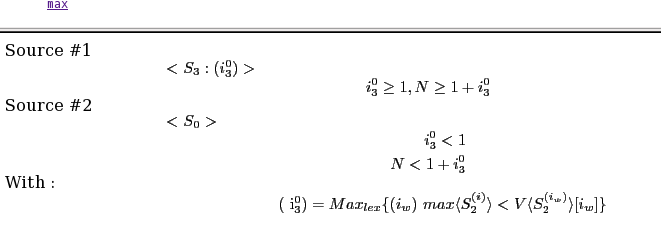
\includegraphics[scale=0.60]{html_tex.png}
\end{center}
\caption{HTML Output for the example of Figure~\ref{pgm:max_vect}}
\label{output:html}
\end{figure}

Here the source of a variable is given in a flat way: the source operation followed by the condition of its validity. The condition is normalised in a DNF form, disjunction (lines) of conjunctions (conjunction of inequations are in a single line).

For example, value of \verb|max| read by $S_4$ during iteration \verb|i| comes from $S_0$ if  $i_3^0 < 1 \vee N < 1 + i_3^0$. This condition ensures that the source is $S_0$ only if no instance of $S_3$ were executed.

For that example, \verb|FADAtool| was not able to compute the exact source operation. But it gives its exact description : $i_3^0 = max_{lex} \{ ( i_w ) / max \langle S_{2}^{(i)} \rangle  < V \langle S_{2}^{(i_w)} \rangle  [ i_w] \}$.

In fact, $i_3^0$ describes the lexicographic maximum (the last write operation) on a set defined by non affine constraints. Here, $i_w$ is an abstract variable used to define the elements of that set.

The source is the {it last} instance of $S_3$ (the lexicographic maximum of the described set) writing in the variable \verb|max|. Since, this set is described by non affine constraints the source can not be evaluated.
It seems pretty printed, but is indeed more complex to read than what we presented so far.
In fact, all non affine entities (variables and array cells) are tagged by the instance of the operation in which they are referenced.
They look like \verb|V <Operation> [Index]| where:
\begin{itemize}
 \item \verb|<Operation>| the operation that references the concerned entity. It looks like: $S_{ID}^{Instance}$  where $ID$ is the identifier of the statement, and $Instance$ its instance.
\item \verb|[Index]| is the array access index. Non-affine laterals with in the index will be tagged in the same way, in that case tagged expressions may not be readable. \verb|A[B[i]+1]| will be tagged as : \verb|A<operation>[B<operation>[i]+1]|.
\end{itemize}


So $max \langle S_{2}^{(i)}\rangle$ should be read: \verb|max| referenced by the instance $i$ of $S_2$. In the same way $V \langle S_{2}^{(i_w)} \rangle  [ i_w]$ is $V[i_w]$ referenced by the instance $i_w$ of $S_2$ (the if-condition).



%\subsubsection{The Instance Wise Dataflow Graph}
\subsubsection{Output: The Instance Wise Dataflow Graph}
Sources of all read variables can be summarised in an instance wise dataflow graph. The dataflow graph produced by \verb|FADAtool| is generated in a \verb|.dot| format (or a \verb|.vcg| format according to the constant \verb|graph_format| in \verb|constants.h|), then automatically converted (if GraphViz installed) into an image. Currently, there is no other output format, we shall appreciate reporting any special format you want the dependence graph will be represented in. 

Here a part of the dataflow graph for the matrix multiply example (Figure~\ref{pgm:matmul}).
\begin{verbatim}
 $ fadatool -i MatMul.c -gc
\end{verbatim}

\begin{center}
 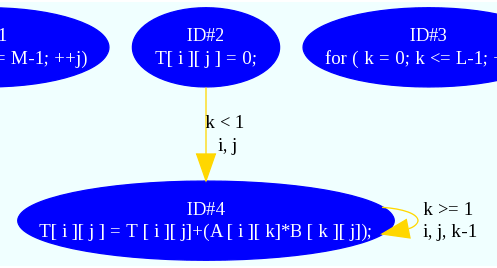
\includegraphics[scale=0.6]{MatMul_DFG.png}
 \end{center}
% \caption{An instance wise dependence graph for program in fig. \ref{pgm:matmul}}
% \label{fig:unfilled_dg}
% \end{figure}

On edges:
\begin{itemize}
 \item The first line gives the condition on validity of the dependence.
 \item The second line gives the function which define the source instance.
\end{itemize}

Here we assume that the read operations are executed during the current iteration vector. Dependent statement instances are identified by an affine function on the read iteration.\\
Let us observe the dependent operations with the operation \verb|ID#4| executed during the iteration \verb|(i, j, k)| (set as the current iteration). One of these dependent operations is \verb|ID#2| executed during the iteration \verb|(i, j)|, the other is another instance of \verb|ID#4| executed during \verb|(i, j, k-1)|.


